\section{Introduction}

\noindent{\bf Motivation and Problem.} A Personal knowledge base enhanced with the information about the users' interpersonal relationships is practical for many applications. For example, relationship facts in a PKB can be accessed by a personalized chat-bot, which will enable it to make better suggestions for the user (for example, suggesting that the user takes her \textit{child} to the zoo instead of a romantic dinner). Moreover, the speech style of the chat-bot, varying from neutral and official to casual and friendly, can be adjusted based on the relationship between the user and her current interlocutor. Finally, if the conversation happens over the phone, the underlying software can automatically assign categories (family/business/..) for the contact list of the user's interlocutors.

With the ubiquity of social media and online forums, user-generated content is available in abundance. Mining personal knowledge from user-generated content to populate PKBs, or \emph{user profiling}, is a long-standing topic in NLP, e.g., \cite{flekova:ACL16:long,basile:2017,tigunova2019listening}. While users' demographic attributes and interests can be learned from their profile descriptions and posts, interpersonal relationships with other users are rarely mentioned explicitly and may only be inferred from their interactions and conversations.

In this work, we develop an automatic method for predicting fine-grained relationships between two speakers, given their logged conversation history.

\begin{figure}[t!]
\centering
\begin{adjustbox}{width=0.46\textwidth}
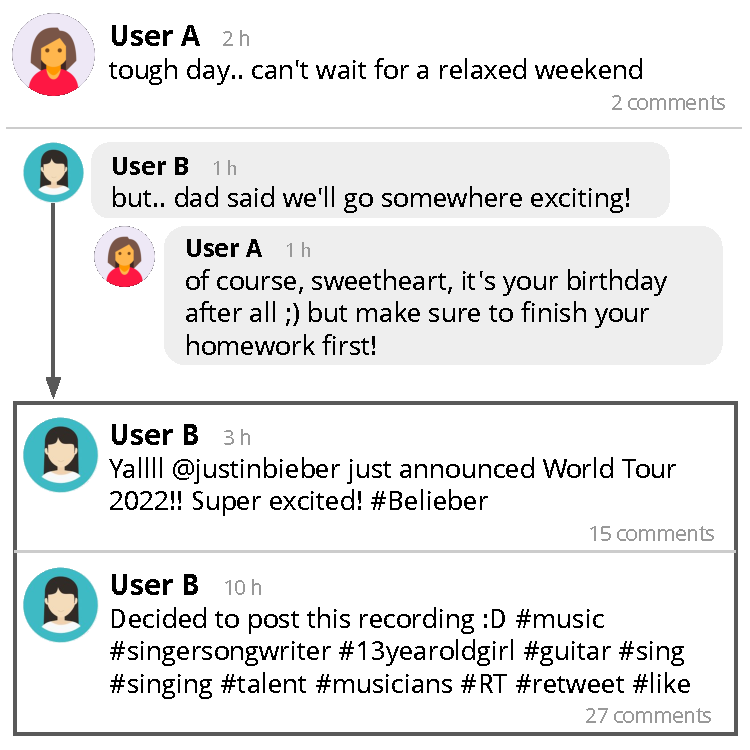
\includegraphics{imgs/conversation_example}
\end{adjustbox}
\caption{Example of two speaker
conversation in social media.}
\label{example_conv}
\end{figure}

Consider the example in Figure~\ref{example_conv}.
From the excerpt of interactions between A and B, the reader can figure out that B is the \textit{child} of A by observing \textit{(i)} the address term `sweetheart', \textit{(ii)} the commanding but soft tone of user A, \textit{(iii)} the reference to the other family member `\textit{dad}', and \textit{(iv)} the context created by the word `\textit{homework}'. Yet, neither of the speakers directly mentions their relationship, making this task difficult for automatic methods 
relying on explicit pattern matching or keyword search.

The relationship information extracted from such conversations, e.g., \textit{<B, child\_of, A>}, can be entered into the PKBs of users A and B. By combining such relationship information with User B's age and personal interests (e.g., \emph{playing guitar, Justin Bieber}) inferable from User B's social media (exemplified in Figure~\ref{example_conv}), 
a system will be able to provide
user A with relevant personalized recommendations for a query ``\textit{birthday present ideas for my daughter}''. 

\paragraphHd{Prior Work and its Limitations.} There has been considerable research on extracting relationships between characters in literary texts such as novels \cite{chaturvedi2016modeling, chaturvedi2017unsupervised}. These methods are inappropriate for conversational data, though, 
which is colloquial and less structured than literary texts. 
Moreover, 
predicting relationships is often  modeled as a binary task of sentiment classification (i.e., person A is positive or negative about person B). 
Prior works on conversational data
are restricted to
small-scale data \cite{yu-etal-2020-dialogue}, or merely handle coarse labels of relationship aspects \cite{rashid2018characterizing,qamar2021relationship}. Most approaches use general models for text classification \cite{chen2020mpdd,jia2020ddrel}, which 
disregard the particularities of
conversational settings. 

\paragraphHd{Approach and Contributions.} We present PRIDE, a 
neural multi-label classifier for \textbf{P}redicting \textbf{R}elationships \textbf{I}n \textbf{D}ialogu\textbf{E}. 
PRIDE makes inference among 12 fine-grained directed relationships (like \emph{child} or \emph{boss}) from conversational data by hierarchically creating utterance representations and combining them with signals on the users' personal attributes (e.g., \textit{age} and \textit{occupation}) and the conversation style (e.g., \textit{intense} or \textit{superficial}).
PRIDE uses BERT \cite{devlin2019bert} to create contextual word embeddings for each utterance, and Transformer encoders \cite{vaswani2017attention} to build conversation representations that preserve information about the sequence and speakers of utterances.

The contributions of this work are: 
\squishlist
\item a method for inferring speakers' relationships from conversational data, which outperforms strong baselines; 
\item an exhaustive analysis of the model's performance. We perform various experiments assessing PRIDE's transfer-learning capabilities and robustness to the varying lengths of the input conversations. Additionally, we conduct ablation studies, proving that all components of the model are essential for the accurate prediction of interpersonal relationships.
\squishend